% Created 2024-10-27 Sun 15:41
% Intended LaTeX compiler: lualatex
\documentclass{beamer}
                

\DeclareExerciseCollection{Concentracoes}
\usetheme{default}
\author{fabio}
\date{\today}
\title{}
\hypersetup{
 pdfauthor={fabio},
 pdftitle={},
 pdfkeywords={},
 pdfsubject={},
 pdfcreator={Emacs 29.4 (Org mode 9.6.15)}, 
 pdflang={English}}
\begin{document}

\begin{frame}{Sumário}
\tableofcontents
\end{frame}



\begin{frame}[label={sec:org8462e63}]{Concentrações}
\begin{block}{Concentração Comum (g/L)}
\begin{itemize}
\item A quantidade de soluto dissolvido num dado volume de solução é denominada de concentração
\item É o quociente entre a massa do soluto e o volume da solução
\item Concentração comum é expressa em \alert{g/L} ou \alert{g L\(^{-1}\)}

\begin{tcolorbox}[ams equation]
\mathcal{C}=\frac{m}{V}
\end{tcolorbox}
\end{itemize}
\end{block}


\begin{block}{Exemplo}
\begin{question}
Qual a massa de cloreto de sódio (NaC\(\ell\)) necessária para preparar 250 mL de uma solução aquosa de concentração igual a 58,5 \unit{\gram\per\litre}.
\end{question}

\begin{answer}[print=true]
\begin{tcolorbox}[ams align*]
\mathcal{C}=& \frac{m_{soluto}}{V_{\text{solu\c{c}\~ao}}} \\
m_{soluto} = & \mathcal{C} \cdot V(mL)_{\text{solu\c{c}\~ao}}\\
m_{soluto}= &  58\;\unit{\gram\per\cancel\litre} \cdot 0,25\; \unit{\cancel\litre}\\
m_{soluto}= & 14,625\; \unit{\gram}
\end{tcolorbox}
\end{answer}
\end{block}

\begin{block}{Concentração molar \(\mathcal{M}\) (mol/L)}
l\#+begin\textsubscript{export} latex
\begin{tcolorbox}[ams align]
\mathcal{M}=\frac{m_{\rm massa\; soluto}}{MM_{massa\;molar} \cdot V_{\text{ solu\c{c}\~ao}}}
\end{tcolorbox}
\#+end\textsubscript{export}

\begin{itemize}
\item Expressa o número de moles do soluto em 1L de solução, sua unidade é \alert{mol/L} ou \alert{\unit{\mole\per\liter}}.
\item A molaridade exprime também o número de milimoles (mmol ou \num{e-3} mol) de um soluto por mililitro (mL ou \num{e-3} L) de solução.

\begin{tcolorbox}[ams equation]
\mathcal{M}=\frac{n_{moles\; soluto}}{V_{\text{solu\c{c}\~ao}}} \Longrightarrow \mathcal{M}=\frac{n_{mmol\; soluto}}{V(mL)_{\text{solu\c{c}\~ao}}}
\end{tcolorbox}

\item Se soubermos a massa do soluto e o volume de solução, podemos calcular a concentração molar.
\end{itemize}
\end{block}

\begin{block}{Exemplo}
\begin{question}
Encontrar a molaridade de uma solução aquosa que contém 2,30 g de álcool
etílico (EtOH; \ch{C2H5OH}) (MM = 46,07 \unit{\gram\per\mole}) em 3,50 L.
\end{question}

\visible<1->{

\begin{answer}[print=true]
\begin{tcolorbox}[ams align*]
\mathcal{M}=& \frac{m_{\rm massa\; soluto}}{MM_{massa\;molar} \cdot V_{\text{ solu\c{c}\~ao}}}\\
\mathcal{M}=& \frac{2,3}{46,07\cdot 3,5}\\
\mathcal{M}=& 0,0143\; \unit{\mol\per\litre}
\end{tcolorbox}
\end{answer}
}
\end{block}

\begin{block}{Relação massa x volume}
\begin{tcolorbox}[ams align]
\%(m/v)=\frac{m}{v_{total}}\cdot 100\% & \quad \text{massa por volume}\\
\%(m/m)= \frac{m}{m_{total}}\cdot 100\% & \quad \text{massa por massa total}\\
\%(v/v)= \frac{v}{v_{total}}\cdot 100\% & \quad \text{volume por volume}
\end{tcolorbox}
\end{block}


\begin{block}{Exemplo I}
\end{block}




\begin{block}{Exemplo II}
\end{block}


\begin{block}{ppm e ppb}
\end{block}


\begin{block}{Exemplo}
\begin{question}
\alert{(UFSCAR-SP)} O flúor tem um papel importante na prevenção e controle da cárie dentária. Estudos demonstram que, após a fluoretação da água, os índices de cáries nas populações têm diminuído. O flúor também é adicionado a produtos e materiais odontológicos. Suponha que o teor de flúor em determinada água de consumo seja 0,9 ppm (partes por milhão) em massa. Considerando a densidade da água 1g/mL, a quantidade, em miligramas, de flúor que um adulto ingere ao tomar 2 litros dessa água, durante um dia, é igual a

\begin{choice}(5)
\choice 0,09.
\choice 0,18.
\choice 0,90.
\choice 1,80.
\choice 18,0
\end{choice}
\end{question}

\begin{answer}[print=true]
\begin{enumerate}
\item Usar a densidade

\begin{align*}
d=\frac{m}{v} \Rightarrow 1 \text{g/mL}=\frac{m}{2000~\text{mL}} \Rightarrow  m = 2000 \; \text{g de \ch{H2O}}
\end{align*}

\begin{enumerate}
\item Cálculo da massa de flúor nesses 2 litros dessa água
\end{enumerate}
\end{enumerate}

\begin{align*}
\frac{0,9\g}{10^6~ \cancel{g}} \cdot 2000~\text{\cancel{g}} \Rightarrow 1,8 \times 10^{-3}~\text{g de F} 
\end{align*}

Isso corresponde a 1,8 mg de  flúor.
\end{answer}
\end{block}


\begin{block}{Diluição de Soluções}
\begin{itemize}
\item As soluções concentradas também podem ser misturadas com solventes para torná-las diluídas.
\item Em diluições a quantidade de solvente é que aumenta e a quantidade de soluto permanece sempre constante. Assim, o número inicial de mols do soluto é igual ao número de mols do soluto no final.mols do soluto no final.
\end{itemize}

\begin{tcolorbox}[ams align]
\mathcal{M}_1 \cdot V_1 = \mathcal{M}_2 \cdot V_2 
\end{tcolorbox}


\begin{center}
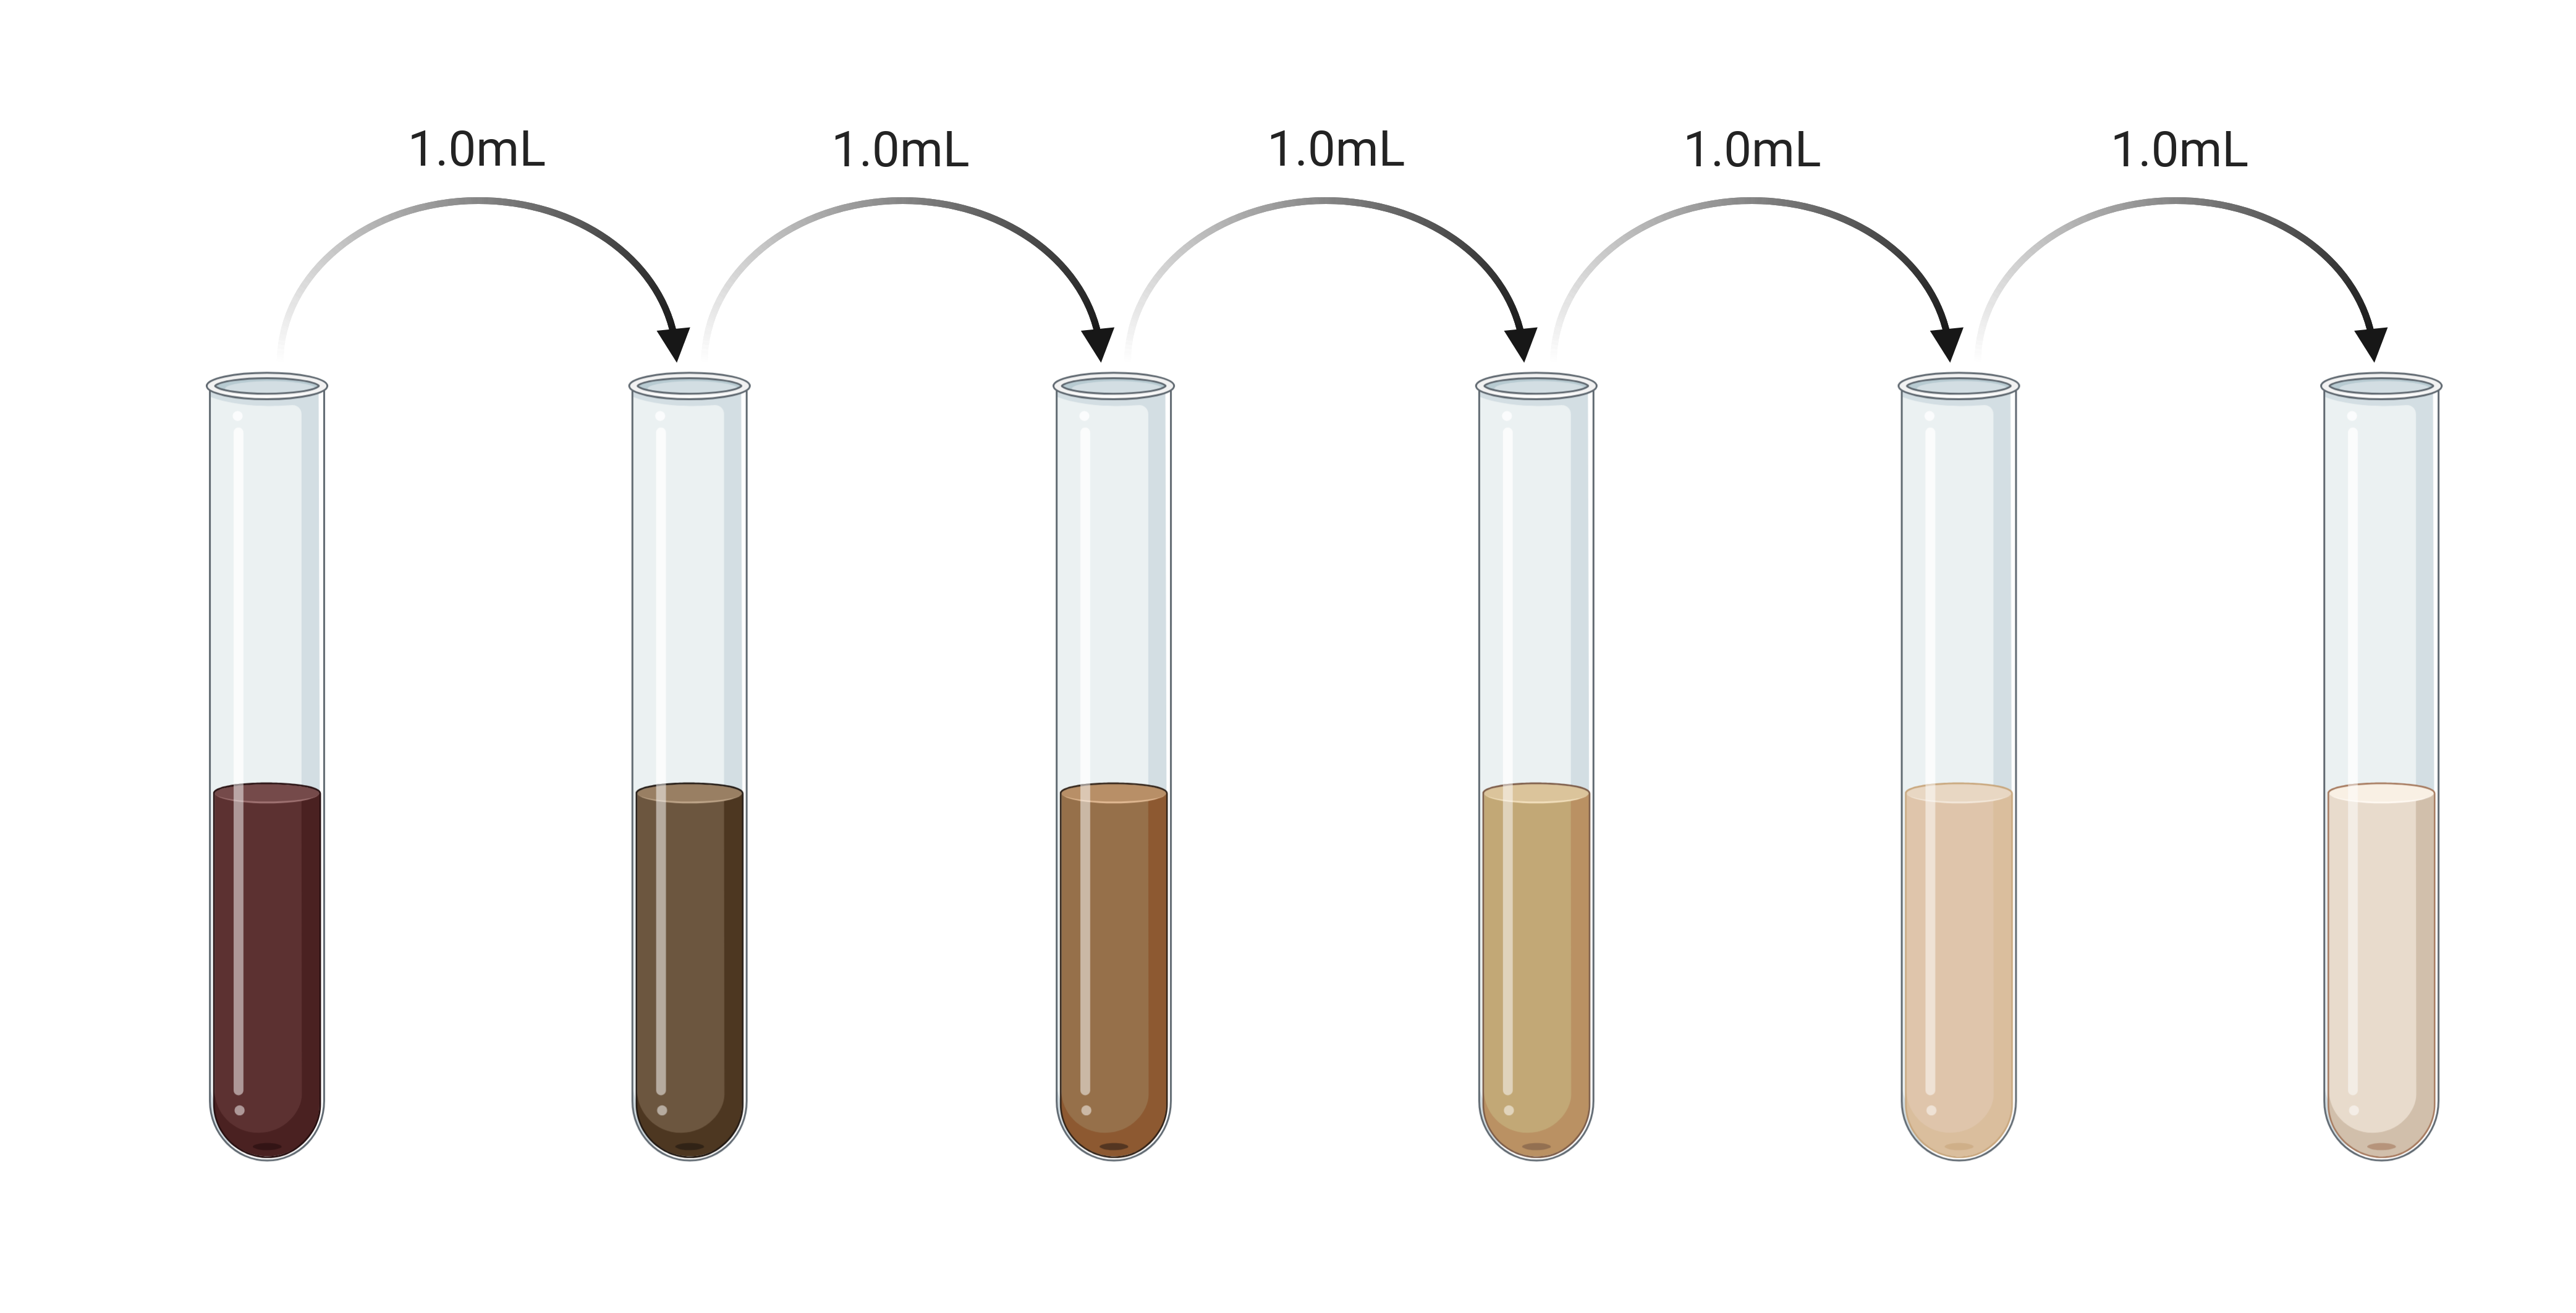
\includegraphics[width=.9\linewidth]{../Solucoes/Diluicao.png}
\end{center}
\end{block}



\begin{block}{Mistura de Soluções}
\begin{itemize}
\item Ocorre quando uma mistura de soluções de mesmo soluto sem reação química consiste em reunir em um mesmo recipiente duas soluções.
\end{itemize}

\begin{tcolorbox}[ams align]
\mathcal{M}_f= \frac{\mathcal{M}_1 \cdot V_1 + \mathcal{M}_2 \cdot V_2}{V_1 + V_2}
\end{tcolorbox}

\begin{center}
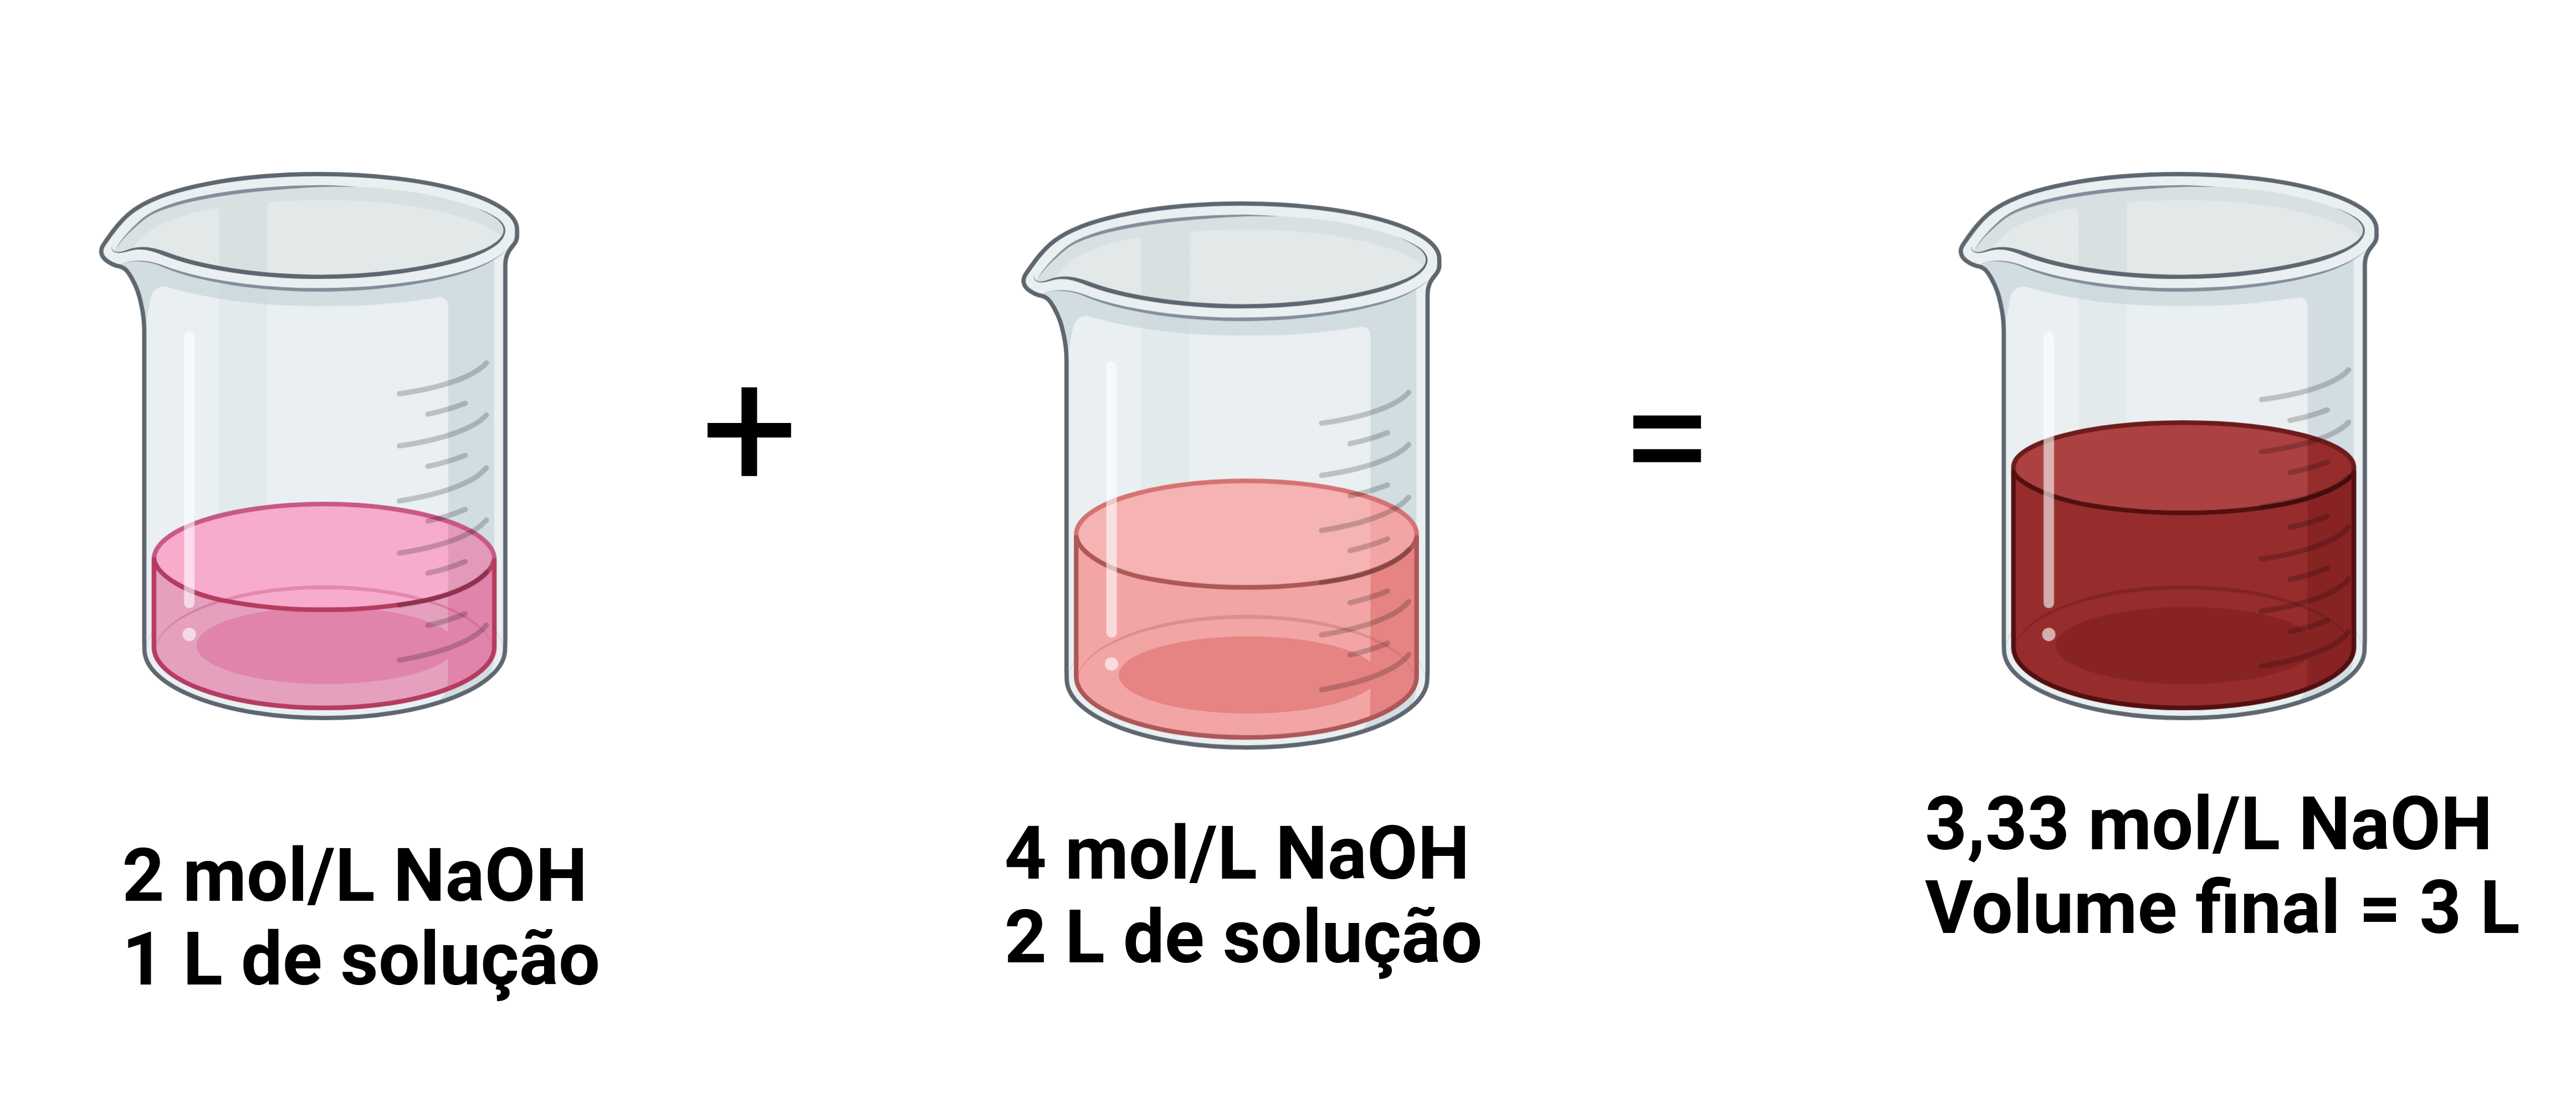
\includegraphics[width=.9\linewidth]{./Mistura_Solucao.png}
\end{center}
\end{block}
\end{frame}
\end{document}
